% Asset ID: AS1DifferentiationTIKZ-003
% Source: Chapter 12 Differentiation PDF p.21 + CCEA AS1-DIFF-LO007
% Related lesson section: Core Theory 14
% Purpose: Show tangent to y=x^2 at (3,9), with equation y-9=6(x-3).

\documentclass[tikz,border=8pt]{standalone}
\usepackage{amsmath}
\usepackage{pgfplots}
\pgfplotsset{compat=1.18}

\begin{document}
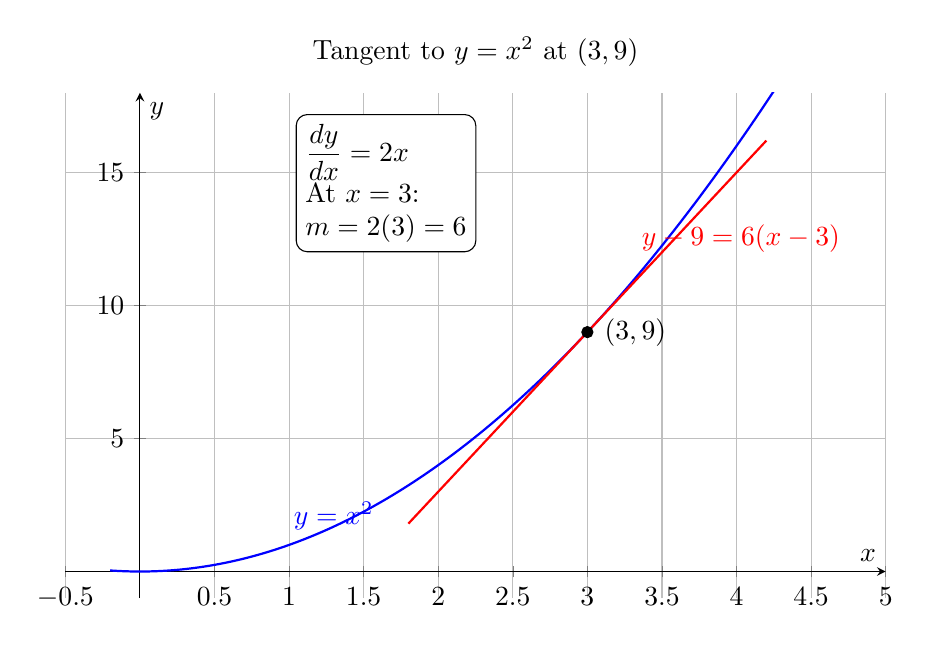
\begin{tikzpicture}
\begin{axis}[
    width=12cm,
    height=8cm,
    axis lines=middle,
    xmin=-0.5, xmax=5,
    ymin=-1, ymax=18,
    grid=both,
    xlabel={$x$},
    ylabel={$y$},
    title={Tangent to $y=x^2$ at $(3,9)$},
    samples=200,
    domain=-0.2:4.5
]
\addplot[thick, blue] {x^2};
\addplot[thick, red, domain=1.8:4.2] {6*(x-3)+9};

\addplot[only marks, mark=*, black] coordinates {(3,9)};
\node[anchor=west] at (axis cs:3.05,9) {$(3,9)$};

\node[blue] at (axis cs:1.3,2.1) {$y=x^2$};
\node[red, anchor=west] at (axis cs:3.3,12.5) {$y-9=6(x-3)$};

\node[fill=white, draw, rounded corners, align=left] at (axis cs:1.65,14.6)
{$\displaystyle \frac{dy}{dx}=2x$\\
At $x=3$:\\
$m=2(3)=6$};

\end{axis}
\end{tikzpicture}
\end{document}
